% ------------------------------------------------------------------------------
% Este fichero es parte de la plantilla LaTeX para la realización de Proyectos
% Final de Grado, protegido bajo los términos de la licencia GFDL.
% Para más información, la licencia completa viene incluida en el
% fichero fdl-1.3.tex

% Copyright (C) 2012 SPI-FM. Universidad de Cádiz
% ------------------------------------------------------------------------------

\section{Metodología de desarrollo}
La metodología usada para el desarrollo de este proyecto es la RUP, conocida como Rational Unified Process en inglés, desarrollada por la empresa
Rational Software propiedad de IBM. Junto con el lenguaje Unificado de modelado UML, constituye la metodología estándar más utilizada para
el análisis, diseño, implementación y documentación de los sistemas orientados a objetos.\\
RUP es un proceso iterativo, centrado en la arquitectura y dirigido por los casos de uso.

\section{Planificación del proyecto}
En este apartado se desarrolla la planificación del proyecto realizando la metodología de desarrollo RUP.\\
Para ver mejor el tiempo de dedicación previsto para las diferentes tareas se incluye un diagrama de Gantt.\\
Resumen de las tareas del proyecto:\\
\begin{itemize}
 \item \textbf{Iniciación}: Esta fase tiene como propósito definir y acordar el alcance del proyecto con los patrocinadores, identificar los riesgos asociados al proyecto, proponer una visión muy general de la arquitectura de software y producir el plan de las fases e iteraciones posteriores.

 \item \textbf{Elaboración}: En la fase de elaboración se estudiarán los casos de uso que permiten definir la arquitectura base del sistema y se desarrollarán en esta fase, se realizará la especificación de los casos de uso seleccionados y el primer análisis del dominio del problema.

\item \textbf{Construcción}: En la fase de construcción se lleva a cabo la construcción del producto por medio de una serie de iteraciones.
Para cada iteración se seleccionan algunos Casos de Uso, se refinan su análisis y diseño y se procede a su implementación y pruebas. Se realiza una pequeña cascada para cada ciclo. Se realizan iteraciones hasta que se termine la implementación de la nueva versión del producto.

 \item \textbf{Documentación}: En esta fase realizaremos la documentación de la memoria.

 \item \textbf{Transición}: En esta fase nos aseguramos que la aplicación funcione correctamente en los usuarios finales. También debemos comprobar que el producto cumpla con las especificaciones aportadas por el cliente y tutor.

Cada fase se completa con la realización de varias iteraciones en las que se desarrollan una serie de actividades, que el modelo RUP clasifica en 9 disciplinas que tienen más o menos importancia en función de lo cerca que se esté o no de la finalización del proyecto.

\begin{itemize}
\item Modelado del negocio. En este conjunto de actividades se persigue el entendimiento de las necesidades de negocio. Documentos de requisitos generales y de alto nivel, reglas del negocio, glosarios, etc. ayudan a definir lo que el producto software deba hacer.
\item Requisitos. Traduce las necesidades del modelo de negocio a requisitos de sistemas automatizables y que con carácter más técnico (se emplean los casos de uso UML), persiguen obtener un entendimiento más profundo del modelo de negocio por parte de los integrantes del equipo de desarrollo.
\item Análisis y diseño. Estas actividades determinan, a partir de los requisitos la arquitectura del sistema más adecuada y el diseño detallado necesario previo a las actividades de implementación.
\item Implementación. Actividades de codificación del software que de acuerdo al diseño, cumplen con los requisitos del sistema.
\item Pruebas. Comprobaciones hechas a todos los elementos que se producen (documentos, diseños o código) para ver que cumplen con los requisitos y con los estándares de calidad definidos para el proyecto.
\item Despliegue. Actividades que permiten tener el sistema instalado en los entornos en que finalmente va a ser explotado.
\item Gestión de configuración. Gestión de los cambios y todos los elementos que intervienen en el proceso de construcción
\item Gestión del proyecto. Actividades encaminadas a la gestión del desarrollo en cuanto a planes, recursos, seguimiento y control y gestión de riesgos.
\item Entorno. Actividades que van encaminadas a dotar al proyecto de recursos hardware y software para facilitar la puesta en marcha y mantenimiento de los distintos entornos de desarrollo y pruebas o la propia puesta en producción del sistema.
\end{itemize}

\subsection{Iteraciones}
\begin{itemize}
\item \textbf{Primera iteración: Edificación del software}\\
Se construyó un prototipo de la aplicación de acuerdo con las necesidades del cliente. Estas necesidades se obtuvieron en las distintas reuniones iniciales.\\
\item \textbf{Segunda iteración: Control de identificación}\\
Se creó un sistema de control de usuarios para que cada tipo de usuario de la aplicación sólo pudiese realizar algunas acciones de acuerdo a sus funciones o responsabilidades.\\
\item \textbf{Tercera iteración: Aumento de funcionalidades}\\
Se aumentaron las funcionalidades del software conforme a las nuevas peticiones del cliente. Se construyó un sistema de citas e informes.\\
\item \textbf{Cuarta iteración: Modificación de base de datos}\\
Se modificó en la base de datos algunos atributos, tanto insertando como eliminando de las tablas. Se modificaron algunos tipos de relaciones.\\
\item \textbf{Quinta iteración: Aumento de las funcionalidades}\\
Se aumentaron las funcionalidades del sistema con la generación de gráficas, auditoría, conexiones de los usuarios al sistema y generación de documentos PDF.\\
\item \textbf{Sexta iteración: Modificación de la interfaz}\\
Se modificó la interfaz de usuario para que se visualizase correctamente en resoluciones de pantalla pequeñas. También se modificó para dotar al sistema de un aspecto más profesional.

\end{itemize}
 
\end{itemize}
\newpage
\begin{figure}[H]
  \centering
    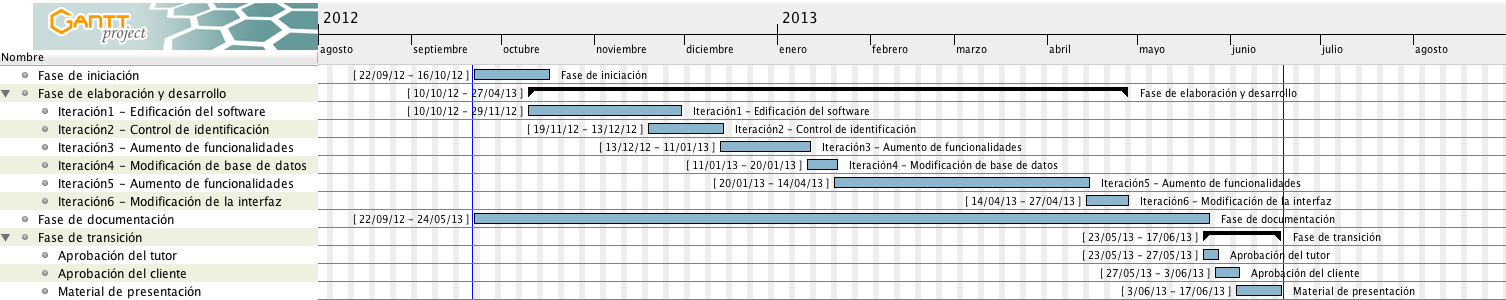
\includegraphics[angle=270,totalheight=22cm,width=8cm]{gantt}
  \caption{Diagrama de Gantt}
  \label{Figura}
\end{figure}

Se realizó la planificación de los tiempos de las tareas pero no se cumplieron debido a problemas no esperados o dificultad añadida no prevista.

\begin{table}[ht]
\centering  % used for centering table
\begin{tabular}{c c c} % centered columns (4 columns)
\hline\hline                        %inserts double horizontal lines
Fase & Tiempo estimado & Tiempo real \\ [0.5ex] % inserts table 
%heading
\hline                  % inserts single horizontal line
Fase de iniciación & 60 horas & 75 horas  \\ % inserting body of the table
Fase de elaboración y construcción & 400 horas & 550 horas \\
Fase de documentación & 30 horas &  50 horas\\
Fase de transición & 50 horas & 70 horas  \\ [1ex]      % [1ex] adds vertical space
\hline %inserts single line
\end{tabular}
\caption{Tiempo estimado - Tiempo real} % title of Table
\end{table}

\section{Organización}
Las personas involucradas en el proyecto son el tutor, el cliente y el desarrollador de la aplicación. El cliente es el que establece cuales son los requisitos y necesidades que quiere para su software mientras que el tutor es el que supervisa progresivamente que llevamos a cabo de forma correcta el proyecto.\\
Los recursos utilizados en el proyecto son un ordenador personal en el entorno de desarrollo y un servidor web donde alojaremos la aplicación. Todo el software usado es software libre por lo tanto no cabe destacar ningún coste salvo el tiempo empleado en desarrollar la aplicación.

\section{Costes}
\begin{itemize}
\item Costes humanos:
\end{itemize}
Para el cálculo de los costes humanos, se han utilizado las tablas salariales para figuras de personal investigador, contratado para el desarrollo de 
proyectos de investigación científica o técnica a través del contrato por obra y servicio aprobadas en 2012. En el documento alojado en la web\footnote{\url{http://www.uca.es/recursos/doc/Unidades/Area_Personal/Capitulo_VI/1143959322_942012113011.pdf}. \textit{Tablas salariales}}, se puede ver como el coste total anual de un ingeniero técnico son 23.237,88 y si calculamos la proporción por el tiempo de duración del proyecto que han sido 745 horas, aproximadamente 5 meses de dedicación el cual tiene un coste de 9.682,45 euros.
\begin{itemize}
\item Costes de materiales:
\end{itemize}
Todas las herramientas que se han usado e instalado son gratuitas y están instaladas en un sistema operativo Ubuntu 12.04.2 LTS, es decir, tanto el software utilizado como el sistema operativo son software libre y por lo tanto no representan ningún coste.

\newpage
\section{Gestión de riesgos}
La Gestión de riesgos es un enfoque estructurado para manejar la incertidumbre relativa a una amenaza, a través de una secuencia de actividades humanas que incluyen evaluación de riesgos, estrategias de desarrollo para manejarlo y mitigación del riesgo.\\
En esta sección describiremos mediante una tabla los riesgos del proyecto %\ref{Riesgos}:
\\
\begin{table}[ht]
\centering  % used for centering table
\begin{tabular}{c c c} % centered columns (4 columns)
\hline\hline                        %inserts double horizontal lines
Riesgo & Probabilidad & Impacto \\ [0.5ex] % inserts table 
%heading
\hline                  % inserts single horizontal line
Tiempo estimado demasiado pequeño & 70\% & 1 semana  \\ % inserting body of the table
Cliente cambia requisitos & 50\% & 1 semana \\
Falta experiencia en herramientas & 60\% & 2 semanas \\
Falta experiencia en planificación & 70\% & 1 semana \\
Falta experiencia en óptica & 80\% & 2 semanas  \\ [1ex]      % [1ex] adds vertical space
\hline %inserts single line
\end{tabular}
\label{Riesgos} % is used to refer this table in the text
\caption{Riesgos} % title of Table
\end{table}

Para disminuir los riesgos se tomaron varias citas con el cliente para definir bien los requisitos, se intentó tener buena experiencia en las herramientas para no entrar en los riesgos y se intentó hacer una buena planificación de los tiempos de las tareas.\\
El tiempo de la tarea aumentaría con cualquiera de los riesgos anteriormente citados.
